\documentclass[english,man]{apa6}

\usepackage{amssymb,amsmath}
\usepackage{ifxetex,ifluatex}
\usepackage{fixltx2e} % provides \textsubscript
\ifnum 0\ifxetex 1\fi\ifluatex 1\fi=0 % if pdftex
  \usepackage[T1]{fontenc}
  \usepackage[utf8]{inputenc}
\else % if luatex or xelatex
  \ifxetex
    \usepackage{mathspec}
    \usepackage{xltxtra,xunicode}
  \else
    \usepackage{fontspec}
  \fi
  \defaultfontfeatures{Mapping=tex-text,Scale=MatchLowercase}
  \newcommand{\euro}{€}
\fi
% use upquote if available, for straight quotes in verbatim environments
\IfFileExists{upquote.sty}{\usepackage{upquote}}{}
% use microtype if available
\IfFileExists{microtype.sty}{\usepackage{microtype}}{}

% Table formatting
\usepackage{longtable, booktabs}
\usepackage{lscape}
% \usepackage[counterclockwise]{rotating}   % Landscape page setup for large tables
\usepackage{multirow}		% Table styling
\usepackage{tabularx}		% Control Column width
\usepackage[flushleft]{threeparttable}	% Allows for three part tables with a specified notes section
\usepackage{threeparttablex}            % Lets threeparttable work with longtable

% Create new environments so endfloat can handle them
% \newenvironment{ltable}
%   {\begin{landscape}\begin{center}\begin{threeparttable}}
%   {\end{threeparttable}\end{center}\end{landscape}}

\newenvironment{lltable}
  {\begin{landscape}\begin{center}\begin{ThreePartTable}}
  {\end{ThreePartTable}\end{center}\end{landscape}}

  \usepackage{ifthen} % Only add declarations when endfloat package is loaded
  \ifthenelse{\equal{\string man}{\string man}}{%
   \DeclareDelayedFloatFlavor{ThreePartTable}{table} % Make endfloat play with longtable
   % \DeclareDelayedFloatFlavor{ltable}{table} % Make endfloat play with lscape
   \DeclareDelayedFloatFlavor{lltable}{table} % Make endfloat play with lscape & longtable
  }{}%



% The following enables adjusting longtable caption width to table width
% Solution found at http://golatex.de/longtable-mit-caption-so-breit-wie-die-tabelle-t15767.html
\makeatletter
\newcommand\LastLTentrywidth{1em}
\newlength\longtablewidth
\setlength{\longtablewidth}{1in}
\newcommand\getlongtablewidth{%
 \begingroup
  \ifcsname LT@\roman{LT@tables}\endcsname
  \global\longtablewidth=0pt
  \renewcommand\LT@entry[2]{\global\advance\longtablewidth by ##2\relax\gdef\LastLTentrywidth{##2}}%
  \@nameuse{LT@\roman{LT@tables}}%
  \fi
\endgroup}


  \usepackage{graphicx}
  \makeatletter
  \def\maxwidth{\ifdim\Gin@nat@width>\linewidth\linewidth\else\Gin@nat@width\fi}
  \def\maxheight{\ifdim\Gin@nat@height>\textheight\textheight\else\Gin@nat@height\fi}
  \makeatother
  % Scale images if necessary, so that they will not overflow the page
  % margins by default, and it is still possible to overwrite the defaults
  % using explicit options in \includegraphics[width, height, ...]{}
  \setkeys{Gin}{width=\maxwidth,height=\maxheight,keepaspectratio}
\ifxetex
  \usepackage[setpagesize=false, % page size defined by xetex
              unicode=false, % unicode breaks when used with xetex
              xetex]{hyperref}
\else
  \usepackage[unicode=true]{hyperref}
\fi
\hypersetup{breaklinks=true,
            pdfauthor={},
            pdftitle={Beyond Overall Effects: A Bayesian Approach to Finding Constraints Across A Collection Of Studies In Meta-Analysis},
            colorlinks=true,
            citecolor=blue,
            urlcolor=blue,
            linkcolor=black,
            pdfborder={0 0 0}}
\urlstyle{same}  % don't use monospace font for urls

\setlength{\parindent}{0pt}
%\setlength{\parskip}{0pt plus 0pt minus 0pt}

\setlength{\emergencystretch}{3em}  % prevent overfull lines

\ifxetex
  \usepackage{polyglossia}
  \setmainlanguage{}
\else
  \usepackage[english]{babel}
\fi

% Manuscript styling
\captionsetup{font=singlespacing,justification=justified}
\usepackage{csquotes}
\usepackage{upgreek}



\usepackage{tikz} % Variable definition to generate author note

% fix for \tightlist problem in pandoc 1.14
\providecommand{\tightlist}{%
  \setlength{\itemsep}{0pt}\setlength{\parskip}{0pt}}

% Essential manuscript parts
  \title{Beyond Overall Effects: A Bayesian Approach to Finding Constraints
Across A Collection Of Studies In Meta-Analysis}

  \shorttitle{Beyond Overall Effects}


  \author{Author(s) Redacted\textsuperscript{1}}

  \def\affdep{{""}}%
  \def\affcity{{""}}%

  \affiliation{
    \vspace{0.5cm}
          \textsuperscript{1} Institution(s) Redacted  }

  \authornote{
    \newcounter{author}
    Author Notes redacted

                        }


  \abstract{Most meta-analyses focus on meta-analytic means, testing whether they
are significantly different from zero and how they depend on covariates.
This mean is difficult to defend as a construct because the underlying
distribution of studies reflects many factors such as how we choose to
run experiments. We argue that the fundamental questions of
meta-analysis should not be about the aggregated mean; instead, one
should ask which relations are stable across all the studies. In a
typical meta-analysis, there is a preferred or hypothesized direction
(e.g., that violent video games increase, rather than decrease,
agressive behavior). We ask whether all studies in a meta-analysis have
true effects in a common direction. If so, this is an example of a
stable relation across all the studies. We propose four models: (i) all
studies are truly null; (ii) all studies share a single true nonzero
effect; (iii) studies differ, but all true effects are in the same
direction; and (iv) some study effects are truly positive while others
are truly negative. We develop Bayes factor model comparison for these
models and apply them to four extant meta-analyses to show their
usefulness.}
  \keywords{meta-analysis, random-effects meta-analysis, Bayesian models, mixed
models, order-constrained inference \\

    
  }




  \usepackage{bm}
  \usepackage{pcl}
  \usepackage{amsmath}
  \usepackage{setspace}

\usepackage{amsthm}
\newtheorem{theorem}{Theorem}
\newtheorem{lemma}{Lemma}
\theoremstyle{definition}
\newtheorem{definition}{Definition}
\newtheorem{corollary}{Corollary}
\newtheorem{proposition}{Proposition}
\theoremstyle{definition}
\newtheorem{example}{Example}
\theoremstyle{remark}
\newtheorem*{remark}{Remark}
\begin{document}

\maketitle

\setcounter{secnumdepth}{0}



Most readers at some point have considered the validity of averages.
Sometimes, we may have been asked, \enquote{What does this average
mean?} or, \enquote{Who does this average describe?} We may be quick to
to gloss over such questions. After all, the average, or sample mean, is
a natural measure of the central tendency, and central tendency holds a
privileged place in understanding variability.

Yet answers based on naturalness and privilege can be unsatisfying. A
better account of the average comes from modeling. A model is an
abstract, platonic account that has an irreducible element of
uncertainty. According to the model, observations come from a
distribution that captures this uncertainty. Part of our goal as
analysts is to characterize this distribution. Unlike the data, which
are real, the distribution is itself an abstraction (de Finetti, 1974).
We often say observations are samples from a distribution. The reader,
however, should keep in mind that this saying is somewhat misleading:
Although observations are real, the concept of a sample from a
distribution is an abstraction.

We may profitably view the sample mean in this context. The sample mean
is useful in characterizing this abstract distribution. If we go further
and assume that the observations come from a common distribution, say
the normal distribution, the sample mean serves as an estimator of
another abstraction, a parameter. For the normal, this parameter is
called the true mean. Although we use the term \enquote{true,} we should
be careful to remember that it is not real quantity---rather, it is a
mathematical abstraction.\footnote{Some people use the term population
  mean rather than true mean. The population is an abstraction, for
  example, the population of all people is an abstract concept not
  dependent on who is currently alive.} Even though parameters are
abstractions rather than real, they are nonetheless useful in
understanding constraint in data. In this regard, the sample mean is
validated as an estimator of a theoretically meaningful parameter in a
model.

One area where this validation seems hollow, however, is meta-analysis.
The usual goal of meta-analysis is to combine several similar studies to
draw a common conclusion. This conclusion almost always centers on a
grand mean or overall effect. Take, for example, the meta-analysis of
Anderson et al. (2010). After an extensive review, these authors
concluded the meta-analytic average of the link between violent video
game exposure and subsequent aggressive behavior was \(r=.21\). Yet, to
interpret this meta-analytic mean, we need to posit a distribution over
experiments and treat this average as an estimate of a true parameter.
The critical problem is this: what does this distribution signify? The
distribution surely has something to do violent-video game exposure and
aggression, but it also has something to do with how we design, run, and
select experiments. In this light, this distribution may be as
appropriate for understanding the sociology of how researchers choose
experiments as it is for understanding the link between violent video
games and aggression. Moreover, even if we generalize from a current set
of studies to new sets, these new sets may be run with different design
parameters and these differences in design may depend on the results of
the previous studies. At the core of the problem, there is no sampling
process from which experiments arise, and because of this, the concept
of a meta-analytic distribution and meta-analytic means must be treated
with much care.

We need not throw out the baby with the bathwater. To make progress, we
distinguish between \emph{metric} and \emph{ordinal} properties. The
metric properties are the usual real-valued parameters that describe the
exact location of the probability mass, including the mean, variance,
quantiles, and moments. For the Anderson et al. meta-analysis, the value
\(r=.21\) is a metric property describing the central tendency of the
distribution of effect sizes across studies. For the reasons stated
above, we consider metric properties of questionable value as the
justification for the distribution they describe is strained.

Ordinal properties, in contrast, are about orderings. We ask whether
basic ordering relations hold across all studies. To start, we note that
there is almost always an anticipated direction of relations or effects
in meta-analysis. For example, if there is an effect of violent video
games on aggressive behavior, theory predicts that such violent video
games are positively associated, rather than negatively associated, with
aggression. We call this anticipated direction the positive direction,
and note that effects may be classified as positive, null, or negative.
We propose that although metric properties of distributions across
experiments may not be meaningful, ordinal properties of negative, null,
and positive are. Here is how: We ask whether all studies in a
population of studies have the same ordinal properties.

For example, we may expect that if there is a positive effect between
aggression and violent video games, all studies with competent methods
and measurements will have a true positive effect. This is not to say
that every study will yield a positive sample effect, as some negative
sample effects are expected from sample noise. Once this noise is
modeled, the resulting parameters may be called \emph{true effects}.
They denote the noise-free or population value of the study, and we will
use the terms \emph{true} and \emph{truly} throughout to refer to these
values as not to confuse them with sample or observed values.The
constraint we study is whether all true effects across a class of
studies are positive. This all-studies-positive constraint, if it holds,
is a strong statement. It means that every experiment in the class has a
true positive effect. It is stronger than the usual meta-analytic
statement about the averages because it applies to all studies.
Likewise, we can also define a strong null constraint---all studies in
the class show a true null effect. This null is stronger than the usual
null that the average across studies is zero as the average may be zero
while constituent studies may be truly positive and negative.

Of course, it may not be that all studies in a corpus have true positive
effects or that all have a true null or that all have a true negative
effect. Perhaps some studies in the meta-analysis show a true positive
effect while others show a true negative effect. This case, should it
exist, motivates different considerations. If there is a mix of true
positive and true negative effects across studies, it may indicate that
the individual studies are measuring disparate phenomena or are
confounded by some moderator that is powerful enough to change the sign
of the true effect. In this case, researchers may want to study why some
effects are truly positive and others are truly negative.

We believe this focus on ordinal properties that are common across all
studies matches well with the type of questions researchers are
interested in. Do all studies show a true effect in the same direction?
Do all studies show a true null effect? Is the effect so heterogeneous
that some studies have a true positive and others have a true negative
effect? The meta-analytic mean, while convenient, is not helpful in
answering these questions. Our goal here is to develop models of these
meta-analytic ordinal constraints. We do so and illustrate a variety of
patterns in the literature by reanalyzing four extant meta-analyses. One
constraint we document is a strong null where all studies have a
zero-valued true effect. We find this constraint holds in a reanalysis
of Wagenmakers et al. (2016). These authors performed a registered
replication of Strack, Martin, \& Stepper (1988), who demonstrated a
well-cited instance of embodied cognition. A second constraint we
document is one where all studies in the meta-analysis are best
described as having one true effect. We document this common effect with
a reanalysis of a set of studies from Ebersole et al. (2016). These
authors replicated a social-psychological phenomenon called moral
credentialism (Monin \& Miller, 2001) where prejudice is expressed to a
greater degree after participants reject overtly sexist statements. A
third constraint we document is one where true effects may differ but
all are positive. This case comes from a reanalysis of Haaf \& Rouder
(2017), who reported the results of three extant Stroop experiments.
Finally, we document unconstrained variability across studies. This is
demonstrated by a reanalysis of Corker, Donnellan, Kim, Schwartz, \&
Zamboanga (2017), who studied how Big Five personality characteristics
varied across different university populations.

Many of the highest visibility developments in meta-analysis today are
about accounting for publication bias in computing and testing
meta-analytic averages (Assen, Aert, \& Wicherts, 2015; Carter,
Schonbrodt, Hilgard, \& Gervais, 2017; Simonsohn, Nelson, \& Simmons,
2014; Stanley \& Doucouliagos, 2014). Because we address a more
fundamental question---what are the constraints among individual
studies---we focus here on basic development without worrying about
publication bias at this juncture.

\section{Constraints Among True
Effects}\label{constraints-among-true-effects}

\begin{figure}[htbp]
\centering
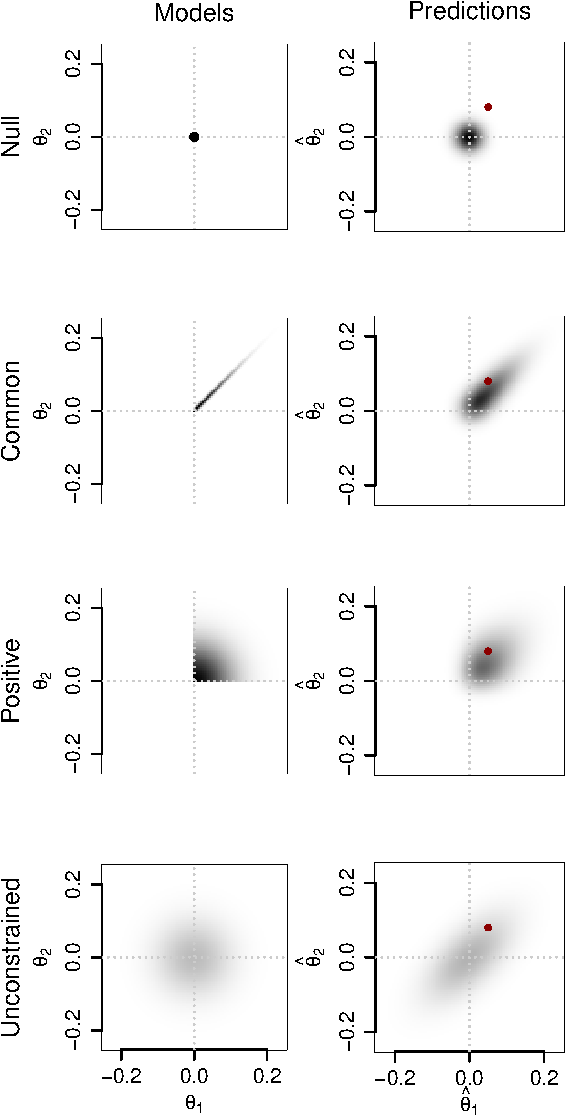
\includegraphics{pBlind_files/figure-latex/pred-1.pdf}
\caption{\label{fig:pred}The four meta-analytic models as shown for two
hypothetical studies. The left column shows the specifications; the
right column shows the resulting predictions on observed effects.}
\end{figure}

Our main goal is to focus on constraints among the constituent
experiments themselves. We first illustrate this focus with a reanalysis
of Wagenmakers et al. (2016). Participants were asked to rate how
humorous cartoons were while either smiling or pouting. Strack et al.
(1988) reported a sizable effect where participants rated the cartoons
as more humorous when smiling than when pouting. Wagenmakers et al.'s
replication set is comprised of data from 17 independent lab sites who
each performed the exact same experiment.

We explicitly model the variability within and between the studies with
an ordinary mixed linear model. Let \(Y_{ijk}\) denote the rating from
the \(i\)th site, the \(j\)th condition, and the \(k\)th participant.
For example in the Wagenmakers' set, there are \(I=17\) studies, two
conditions (pout and smile, \(j=1,2\), respectively), and about 60
replicates per study per condition. The base model is \[
Y_{ijk} = \mu+\alpha_i + x_j\theta_i+\epsilon_{ijk}.
\] Here, \(\mu\) is a grand mean and \(\alpha_i\) is an overall
study-specific effect. Studies with higher ratings on average will have
greater values of \(\alpha_i\). In this regard, \(\alpha_i\) is a
study-specific \emph{intercept} parameter. The design element \(x_j\) is
a condition indicator with \(x_j=-1/2\) and \(x_j=1/2\) for pout and
smile conditions, respectively. The parameter \(\theta_i\) is the
study-specific effect of the pout/smile manipulation, and it is the main
target of inquiry. These parameters may be thought of as study-specific
\emph{slopes} as they describe the study-specific change in performance
as a function of the manipulation. The term
\(\epsilon_{ijk}\stackrel{iid}{\sim}\mbox{Normal}(0,\sigma^2)\) is the
usual noise term.

Our critical questions are about \(\theta_i,\) the effect of the
smile/pout manipulation. To address these questions, we place a series
of models on \(\theta_i\) that capture various constraints:

The most constrained model is the \emph{null model}. Here, all of the
constituent studies have a true effect of zero, and this model is
implemented with the constraint \(\theta_i=0\). Note that this model is
a much stronger null than the usual meta-analytic null where the true
grand average is zero; here, both the average and variance of
\(\theta_i\) are zero. Figure~\ref{fig:pred}, left column, provides a
graphical representation of the models. Panel A is for the null model.
Depicted is the specification of the effect \(\theta_i\) for two
studies. Since \(\theta_i\) is zero for both studies, the only point
with mass is at \((0,0)\).

The next generalization is what we term a \emph{common effect model}.
All constituent studies have the same true value, denoted \(\nu\). The
constraint is simply \(\theta_i=\nu\). This one-effect model captures
the assumption of homogeneity sometimes stipulated in fixed-effect
meta-analysis (Borenstein, Hedges, Higgins, \& Rothstein, 2010).
Figure~\ref{fig:pred}B depicts this model. Because of the equality
constraint, there is mass only on the main diagonal. If we further
constrain \(\nu\) to be positive, then there is only mass on positive
values of this diagonal.

A generalization of the common effect model is to allow the true effects
to vary from study-to-study, but to stipulate they have the same
direction. For example, it is reasonable to assume that if facial
expression affects humor ratings, all studies would show, to some
degree, more humorous ratings while smiling than while pouting. Although
that degree may vary, and certain factors may lead to smaller effects
(less-sensitive measurements, less-susceptible populations, noisier
methodology), no study would have a truly negative effect where pouting
led to truly higher humor ratings. We call this model the \emph{positive
effects} model, and with it we constraint \(\theta_i>0\). For example,
\[
\theta_i \sim \mbox{Normal}_+(\mu_\theta,\sigma^2_\theta),
\] where \(\mbox{Normal}_+\) denotes a normal distribution truncated
below at zero. Here \(\mu_\theta\) and \(\sigma^2_\theta\) are
population parameter that describe the distribution of effect sizes
across studies. Figure~\ref{fig:pred}C shows this model. There is only
mass distributed across the quadrant of joint positive effects. Prior
settings are needed for \(\mu_\theta\) and \(\sigma^2_\theta\), and we
discuss how we chose these and the effects of these choices on inference
subsequently.

Finally, we can relax this positivity constraint: \[
\theta_i \sim \mbox{Normal}(\mu_\theta,\sigma^2_\theta).
\] This model is termed the \emph{unconstrained model}, and it specifies
that true effects may be positive or negative. Figure~\ref{fig:pred}D
shows this model, and there is mass across all values of joint effects
across participants.

Some readers might be a tad confused that we previously critiqued
meta-analytic averages and yet still posit parameter \(\mu_\theta\),
which is the meta-analytic average across studies. The difference,
however, is that our focus remains on the collection of \(\theta_i\)'s
and not on \(\mu_\theta\) or \(\sigma^2_\theta\). In this sense, the
experiment-population parameters serve as auxiliary parameters that
improve our estimates of the \(\theta_i\)'s.

These four models provide a means of characterizing the ordinal
constraint in data. For example, if the null model best describes the
data, then the conclusion is that there is no effect for any study.
Likewise if the common-effect model best describes the data, we can talk
about a unified phenomenon, and, here, the mean becomes meaningful as it
characterizes all effect sizes. If the positive model best describes the
data, we may note that while there is variation across studies, all
index the same basic ordinal relation. It is this relation that is the
main constraint in the data. Finally, if the unconstrained model best
describes the data, resulting conclusions are nuanced. Perhaps the most
prudent course is to wonder about the coherence of the collection of
studies---they may index disparate phenomena.

One critical question is which model best describes the obtained data.
We address this question in subsequent sections. Before doing so, we
take a brief detour to discuss estimation of effects. Although
estimation does not provide a calibrated, formal means of assessing the
aforementioned constraints, it certainly provides an appropriate
informal visualization of these constraints, and therefore, obtaining
principled estimates of study effects is consequential.

\section{Estimating True Effects}\label{estimating-true-effects}

A standard course to visualizing effects is a \emph{forest plot}, which
summarizes the sample effect and corresponding confidence interval for
each study or site. Figure~\ref{fig:wagEst}A is an example from
Wagenmakers et al., and it is quite similar to Wagenmakers et al.'s
Figure 4. We find that forest plots place too much emphasis on the
sample means, which, in the case of meta-analysis, are poor estimates of
the true mean.

A sample mean estimate for a certain study relies on the data from that
certain study and not on the data from the other studies in the
meta-analysis. At first glance, this property may seen reasonable, but
since the 1960s, statisticians have known that the data in the other
studies may be used to improve the estimate of a particular study's true
effect size (Efron \& Morris, 1977; Stein, 1956). The estimator for one
study's effect size should depend on the data from that study and from
the other studies as well. This approach is now standard in hierarchical
modeling.

Figure~\ref{fig:wagEst}B shows the hierarchical estimates from the
unconstrained model (filled circles) for Wagenmaker et al.'s data along
with associated 95\% credible intervals. Notice that the hierarchical
estimates are more compact, closer to the meta-analytic average, and
have credible intervals that are smaller and more uniform than for the
sample mean and CIs. This effect is called regularization, and the
notion here is that once the within-study variability is accounted for,
the resulting model estimates better show the true variation across
studies. There is a large degree of regularization; sample mean
estimates are about 3 times as variable as the hierarchical estimates
from the unconstrained model. According to this model, about 1/3 of the
variation in sample estimates may reflect variation across sites; the
other two-thirds may reflect variation within sites. This degree of
regularization is meaningful and substantial.

Plots based on sample effects always overstate the variability across
the sites. To avoid this overstatement, regularization, whether from
frequentist or Bayesian methods, should be used. Sample effects may be
plotted, but they should serve as data rather than as a target of
inference. Consequently, confidence and credible intervals should be
placed on regularized estimates rather than sample means, and
Figure~\ref{fig:wagEst}B provides an example of such a plot.
Fortunately, most researchers are familiar with modern estimation and
mixed linear models, and their usage is built into meta-analytic
software packages such as \texttt{metafor} (Veichtbauer, 2010) and
Comprehensive Meta-Analysis.

\section{Evidence for Constraints}\label{evidence-for-constraints}

Previously, we discussed four theoretically-motivated models of
constraint: the null model, the common effect model, the positive
effects model, and the unconstrained model. Estimating true values for
effects is useful in visualizing data, but it provides no direct and
calibrated measure of the evidence for the four models. To provide
principled measures of evidence, we use the proper Bayesian approach
resulting from Bayes' rule. Rather than providing a formal discourse,
which may be found in Jeffreys (1961), Kass \& Raftery (1995), and
Morey, Romeijn, \& Rouder (2016), we provide an informal discussion that
we have previously presented in Rouder, Morey, \& Wagenmakers (2016) and
Rouder (2017). Informally, evidence for models reflects how well they
predict data.

The right column of Figure~\ref{fig:pred} shows the predictions for each
of the four models. We consider the relationship between two
hypothetical studies that yield sample effects, \(\hat{\theta}_1\) and
\(\hat{\theta}_2\). Possible sample effects for the first experiment are
plotted on the x-axis, and possible values for the second experiment are
plotted on the y-axis. Each point in the figure represents a possible
combination of observed effects. For the null model, the observed
effects are predicted to be near (0,0), and this case is shown in
Figure~\ref{fig:pred}E. The effect of sampling error is to smear the
form of the model.\footnote{More technically, the predictions are the
  integral \(\int_\theta f(Y|\theta)\pi(\theta)d\theta\) where
  \(f(Y|\theta)\) is the probability density of observations conditional
  on parameter values and \(\pi(\theta)\) is the probability density of
  the parameters.} Figures~\ref{fig:pred}F-H show the predictions for
the common effect, positive effects, and unconstrained models,
respectively. One aspect of the predictions that is not obvious is the
correlation for the positive and unconstrained models. This correlation
comes from the hierarchical structure in these models, and is a direct
result of variability of the population mean \(\mu_\theta\). This
variability comes from the prior and is discussed further after
presenting the applications.

Once the predictions are known, model comparison is simple. All we need
to do is note where the data fall. The red dots in the right column
denote a hypothetical observed sample effect for both studies. This
value is about equal for both studies, and we might suspect that the
common effect model does well. To measure how well, we note the density
of the prediction. Here, the density is darkest for the common effect
model. These densities have numeric values, and we may take the ratio to
describe the relative evidence for one model vs.~another. For example,
the best fitting model in the figure, the common effect model, has a
density that is twice the value of that of the positive effects model.
Hence, the data are predicted twice as accurately under the common
effect model than under the positive effects model. This ratio is the
\emph{Bayes factor}, and it serves as the principled measure of evidence
for comparing one model to another in the Bayesian framework.

Bayes factors are conceptually straightforward---one simply computes the
predictive densities at the observed data. While this computation is
conceptually straightforward, it is often inconvenient in practice. The
computation entails the integration of a multidimensional integral which
is often impossible in closed form and may be slow or inaccurate with
numeric methods. To that end, there has been a voluminous literature on
how to compute these integrals in mixed settings such as the one here.
We follow a fairly general set of specification and computations known
to work well. These have been pioneered by Zellner \& Siow (1980) and
expanded for ANOVA by Rouder, Morey, Speckman, \& Province (2012). This
development covers comparisons among the null, common effect, and
unconstrained models. It does not, however, cover comparisons to the
positive effects model. To make these comparisons, we use a different
computational approach from Hoijtink and colleagues (Klugkist \&
Hoijtink, 2007; Klugkist, Kato, \& Hoijtink, 2005). The details are
provided in Haaf \& Rouder (2017).

\section{Prior Settings}\label{prior-settings}

Bayesian analysis is predicated on specifying prior distributions on
parameters. Analysts should be familiar with how these specifications
affect model comparison. A few points of context are helpful. It seems
reasonable as a starting point to require that if two researchers run
the same experiment and obtain the same data, they should reach the same
if not similar conclusions. Yet, almost all Bayesians note that priors
have effects on inference. To harmonize Bayesian inference with the
above starting point, many Bayesian analysts actively seek to minimize
these effects by picking likelihoods, prior parametric forms, and
heuristic methods of inference so that variation in prior settings have
minimal influence (Aitkin, 1991; Gelman, Carlin, Stern, \& Rubin, 2004;
Kruschke, 2012; Spiegelhalter, Best, Carlin, \& Linde, 2002). In the
context of these views, the effect of prior settings on inference is
viewed negatively; not only is it something to be avoided, it is a
threat to the validity of Bayesian analysis.

We reject the starting point above including the view that minimization
of prior effects is necessary or even laudable. Rouder et al. (2016)
argue that the goal of analysis is to add value by searching for
theoretically-meaningful structure in data. Vanpaemel (2010) and
Vanpaemel \& Lee (2012) provide a particularly appealing view of the
prior in this light. Accordingly, the prior is where theoretically
important constraint is encoded in the model. In our case, the prior
provides the critical constraint on the relations among studies. The
choice of prior settings are important because they unavoidably affect
the predictions about data for the models (Figure~\ref{fig:pred}).
Therefore, these settings necessarily affect model comparison. We think
it is best to avoid judgments that Bayes factor model comparisons depend
too little or too much on priors. They depend on it to the degree they
do. Whatever this degree, it is the degree resulting from the usage of
Bayes rule, which in turn mandates that evidence for competing positions
are the degree to which they improve predictive accuracy.

When different researchers use different priors, they will reach
different opinions about the data. Rouder et al. (2016) argue that this
variation is not problematic. They recommend that so long as various
prior settings are justifiable, the variation in results should be
embraced as the legitimate diversity of opinion. When reasonable prior
settings result in conflicting conclusions, we realize the data do not
afford the precision to adjudicate among the positions.

The critical prior specifications are those that define the differences
between the models. In our case, the specifications are on
\(\mu_\theta\) and \(\sigma^2_\theta\), the population parameters.
Although these parameters are not the primary target of inference, the
prior settings on them affect the resulting Bayes factors. A full
discussion of the prior structures on these parameters is provided in
Haaf \& Rouder (2017), and here we review the main issues. The critical
settings are the \emph{scale} on \(\mu_\theta\) and \(\sigma^2_\theta\).
The scale on \(\mu_\theta\) calibrates the expected size of the effect.
This scale is not a point setting; \(\mu_\theta\) may be free to take on
any value that reflects the data. Figure~\ref{fig:prior}A shows a plot
of the prior on \(\mu_\theta\) for three different scale settings. In
application, we set the scale on \(\mu_\theta\) to be 0.40 in
standardized effect size, and this value corresponds to the middle curve
in the figure, which is dashed. The other setting is the scale of
\(\sigma^2_\theta\), and this setting calibrates the expected amount of
variability in effect size across studies. We chose a value of 0.24
(this is a standard deviation on site-specific standardized effect
sizes). The expected variation across sites or studies is 60\% of the
expected effect size, which seems like a reasonable ratio of scales.
Figure~\ref{fig:prior}B shows a plot of the prior on \(\sigma_\theta\)
for three different scale settings, and the middle one, which is dashed,
corresponds to the value we used.








\begin{figure}[htbp]
\centering
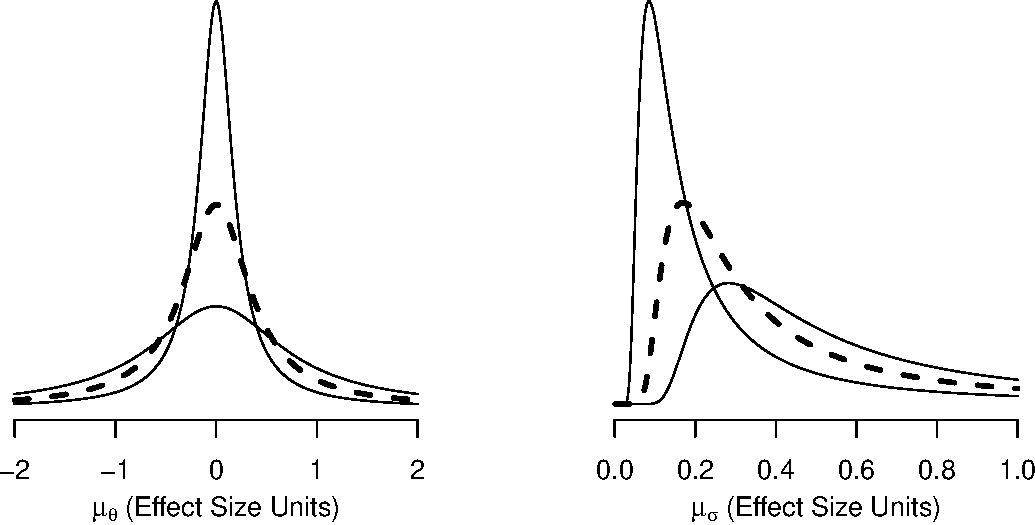
\includegraphics{pBlind_files/figure-latex/prior-1.pdf}
\caption{\label{fig:prior}Prior distributions on critical parameters for different scale
settings. \textbf{A} Priors for \(\mu_\theta\) with scale factors that
range from 0.20 to 0.80. Our choice is the dashed curve for scale value
of 0.40. \textbf{B}. Priors for \(\sigma_\theta\) with scale factors
that range from 0.12 to 0.48. Our choice is the dashed curve for scale
value of 0.24.}
\end{figure}

\section{Wagenmakers et al.'s Embodied
Cognition}\label{wagenmakers-et-al.s-embodied-cognition}

\begin{figure}[htbp]
\centering
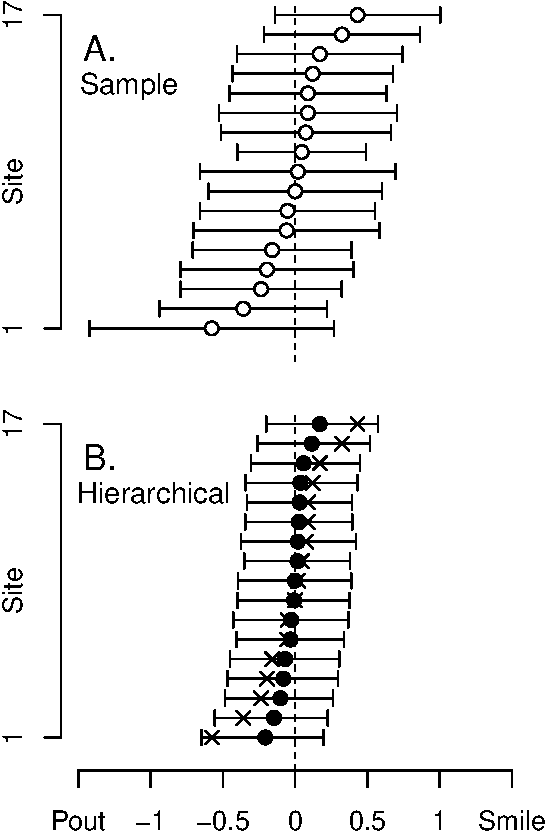
\includegraphics{pBlind_files/figure-latex/wagEst-1.pdf}
\caption{\label{fig:wagEst}Reanalysis of Wagenmakers et al. (2016)
registered replication report. \textbf{A}. Sample means with 95\%
confidence intervals for the 17 sites. \textbf{B}. Hierarchical model
estimates with 95\% credible intervals. These estimates show that after
sample noise is accounted, there is not much heterogeneity.}
\end{figure}

\begin{table}[tbp]
\begin{center}
\begin{threeparttable}
\caption{\label{tab:sens}}
\begin{tabular}{lllll}
\toprule
Mean & \multicolumn{1}{c}{SD} & \multicolumn{1}{c}{Null-to-Common} & \multicolumn{1}{c}{Null-to-Unconstrained} & \multicolumn{1}{c}{Null-to-Positive}\\
\midrule
0.40 & 0.24 & 11.3-to-1 & 261.1-to-1 & 47173.7-to-1\\
0.40 & 0.40 & 11.3-to-1 & 1964.3-to-1 & 2689151.6-to-1\\
0.40 & 0.12 & 11.4-to-1 & 52.8-to-1 & 1620.3-to-1\\
0.80 & 0.48 & 22.2-to-1 & 9929.5-to-1 & Inf-to-1\\
0.80 & 0.80 & 22.3-to-1 & 371027.3-to-1 & Inf-to-1\\
0.80 & 0.24 & 21-to-1 & 504.4-to-1 & 149297.3-to-1\\
0.20 & 0.12 & 5.8-to-1 & 27.1-to-1 & 630.7-to-1\\
0.20 & 0.20 & 5.8-to-1 & 78.1-to-1 & 14582.6-to-1\\
0.20 & 0.06 & 5.8-to-1 & 12.8-to-1 & 82.9-to-1\\
\bottomrule
\addlinespace
\end{tabular}
\begin{tablenotes}[para]
\textit{Note.} Infinite values exceed our machine precision of $10^304$
\end{tablenotes}
\end{threeparttable}
\end{center}
\end{table}

Figure~\ref{fig:wagEst}B provides the results of the reanalysis of
Wagenmakers et al.'s registered replication report. The results from
estimation are highly suggestive that there is no effect among any of
the studies. The Bayes factor analysis favors the null model. The null
is preferred 11-to-1 to the common effect model, the next most preferred
model. The strong null is preferred 250-to-1 and 36,000-to-1 to the
unconstrained and positive effects models, respectively. Here we see
formal support for the strong null model---not only is the
\emph{average} effect nearly zero, but the most parsimonious description
among the four models is that \emph{all} studies have a true zero
effect.

Above we discussed that these Bayes factors are dependent on prior
settings. Our choices of scale for mean and standard deviation are shown
as the middle densities in Figure \ref{fig:prior}. These choices are
informed by general knowledge about the field. We have also provided a
reasonable range of variation in these choices, and these are indicated
by the bracketing densities. We explore the effects of using these
bracketing priors, and the resulting Bayes factors are shown in Table
\ref{tab:sens}. There is a fair amount of variability in Bayes factors,
and in our opinion, there should be. The range of settings define quite
different models with quite different predictions. Nonetheless, there is
a fair amount of consistency. For all settings, the ordering of the
models remain: the null model is preferred to the common effect model
which is preferred to the unconstrained model which is preferred to the
positive effects model. This type of sensitivity analysis can always be
performed to understand the range of conclusions that may be drawn from
the data. In our case, the range is limited to a single ordering.

\section{Ebersole et al.'s Moral Credentialism and
Sexism}\label{ebersole-et-al.s-moral-credentialism-and-sexism}

\begin{figure}[htbp]
\centering
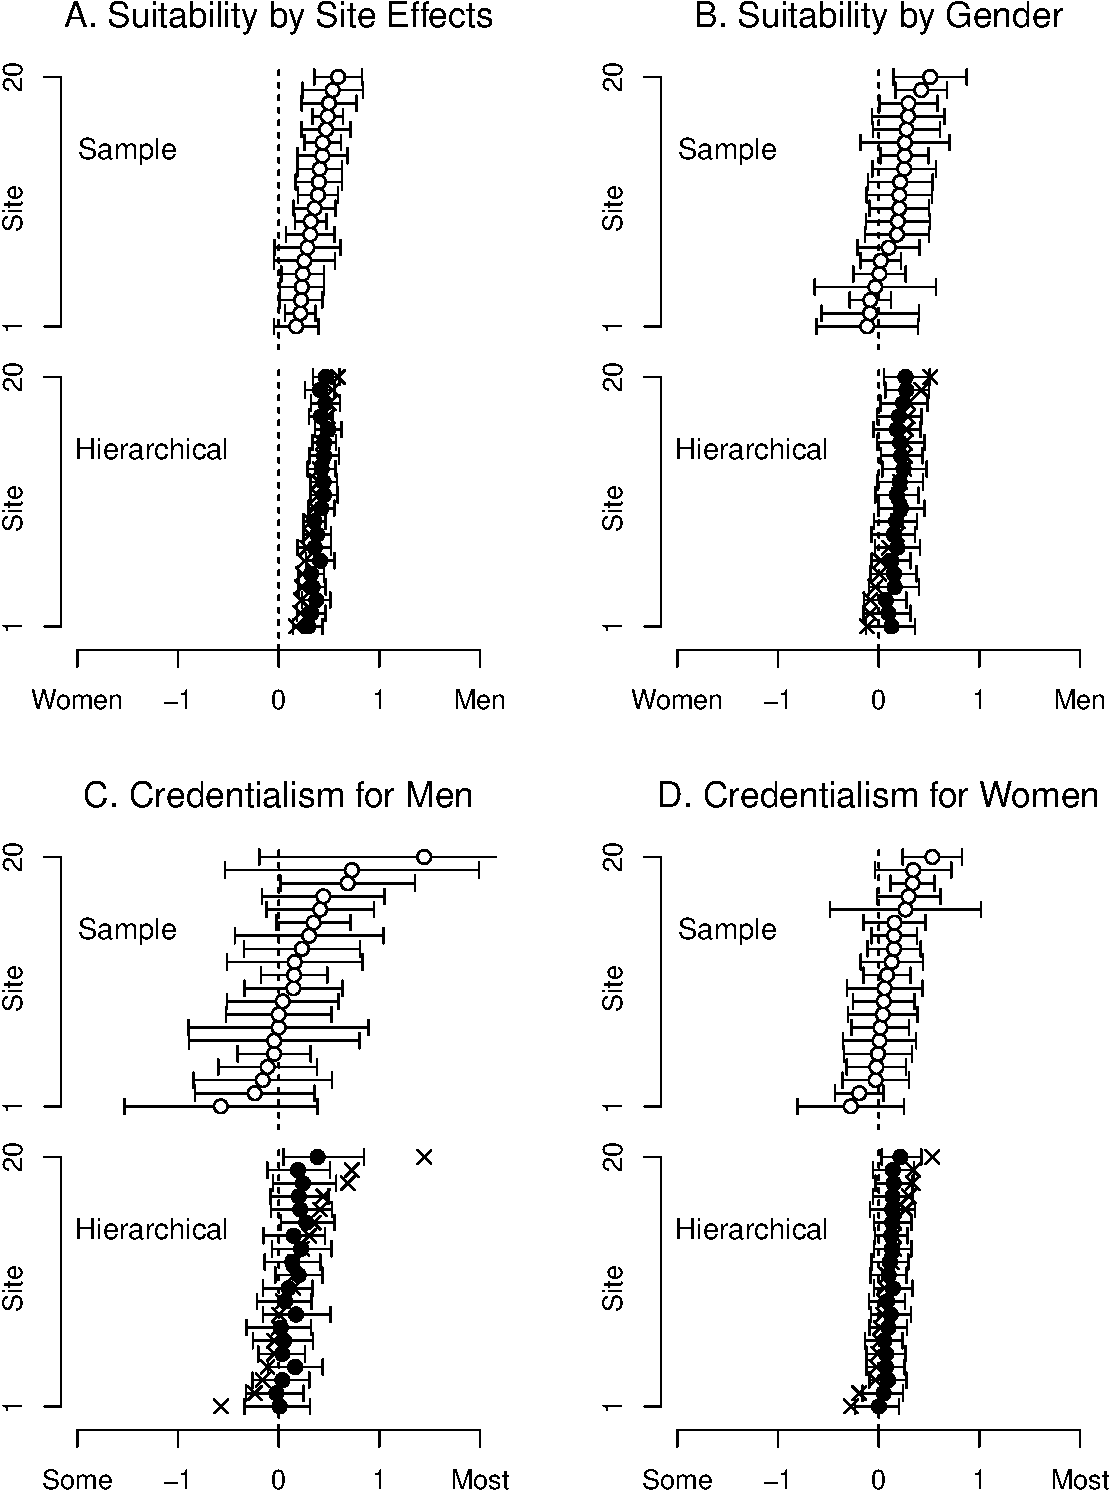
\includegraphics{pBlind_files/figure-latex/ml3Est-1.pdf}
\caption{\label{fig:ml3Est}Reanalysis of Ebersole et al.'s (2016)
replication of the moral-credentialism effect. \textbf{A}. Sample means
with 95\% confidence intervals for the 20 sites. \textbf{B}.
Hierarchical model estimates with 95\% credible intervals. There is
little evidence for heterogeneity across labs.}
\end{figure}

To show how the meta-analytic Bayes factor model-comparison system works
in a more complex example, we re-analyzed a meta-analytic data set from
Ebersole et al. (2016). This paper was the result of the \emph{Many Labs
3 Project}, which was designed to assess the replicability of ten
effects across several sites and across different periods of the
semester. We focus here on one particular effect, \emph{the moral
credential effect,} which was originally demonstrated by Monin \& Miller
(2001).

The Monin and Miller study was designed to assess whether participants
were more likely to express prejudiced attitudes when their prior
behavior suggested that they were not prejudiced. To manipulate prior
behavior, Monin and Miller asked participants to consider sexist
statements and endorse those they agreed with and reject those they did
not. The key manipulation is whether the statement was worded to
describe \emph{most} women or \emph{some} women. The main notion is that
participants would be more likely to reject sexist statements that
described most women rather than some women. Participants were randomly
assigned to the \emph{most} and \emph{some} condition, with those in the
former rejecting more sexist statements than those in the latter. Next,
participants read a vignette that described a hiring opportunity at a
manufacturing company. Participants rated how much more or less suitable
a man would be for the position relative to a woman. The rating scale
was a seven-point scale from strong preference for a woman through
neutral to strong preference for a man.

The main hypothesis is that participants who previously rejected sexist
statements---those who judged sexist statements referring to \emph{most}
rather than \emph{some} women---would be more likely to express that men
are more suitable than women for the job. Indeed, Monin and Miller
report such an effect, and they also report an interaction such that the
effect is prevalent for male participants but not for female
participants.

We specify four critical parameters for each site. There is a
site-specific intercept parameter, denoted \(\alpha_i\) for the \(i\)th
site. This parameter denotes overall rated suitability of men vs.~women
for the hypothetical job opportunity. Variation in this parameter across
sites accounts for variation of overall expression of gender prejudice.
There are three slope parameters to describe the effects. One is a
site-specific gender-of-rater effect parameter, denoted \(\theta_{gi}\).
The gender-of-rater effect is whether male participants rate men
candidates higher than female participants rate men candidates. We refer
to this effect as the gender effect for brevity. The remaining two
parameters represent a moral credential effect---do participants express
more prejudice if they were in the \emph{most}-women condition
previously? Because Monin and Miller reported moderation of this moral
credential effect by gender, we used separate site-specific parameters
for male and female participants, denoted \(\theta_{mi}\) and
\(\theta_{wi}\), respectively. This parameterization is well-suited for
assessing the question whether any credential effect is stronger for men
than for women.

We start with an unconstrained model where all four site-specific
parameters are free to vary subject to a hierarchical structure as used
above.\footnote{A formal statement of the unconstrained model is as
  follows. Let \(Y_{ijk\ell}\) denote the \(\ell\)th replicate for the
  \(i\)th site, \(j\)th gender-of-rater (\(j=1,2\)), and \(k\)th
  credential condition (\(k=1,2\)). The model is given by
  \(Y_{ijk\ell}\sim \mbox{Normal}(\mu_{ijk},\sigma^2)\), where
  \(\mu_{ijk}=\alpha_i +u_j\theta_{gi}+m_{jk}\theta_{mi}+w_{jk}\theta_{wi}\).
  Here \(u_j=-.5,.5\) is an indicator that encodes the gender of the
  rater; \(m_{jk}=0,1\) is an indicator that is 1 if the rater is a man
  and the condition is credentialed (most statements) and 0 otherwise;
  \(w_{jk}=0,1\) is an indicator that is 1 if the rater is a woman and
  the condition is credentialed (most statements) and 0 otherwise.}
These hierarchical structures lead to regularization, and the resulting
estimates for the slope effects are shown in Figure~\ref{fig:ml3Est}.
From these estimates several trends are evident. From
Figure~\ref{fig:ml3Est}A, there is an overall tendency to judge men, as
compared to women, as more suitable for the job. This tendency seems not
to vary among the sites. This tendency is a function of the gender of
the rater: as compared to female participants, male participants are
more likely to rate men higher than women. The gender effect seems to be
stable across sites. Finally, there is a small credential effect for
both men and women.

The figure alone does not lead to calibrated inference. There are many
possible models corresponding to the placement of null, common effect,
positive effects, and unconstrained structures jointly on the four
site-specific variables \(\bfalpha\), \(\bftheta_g\), \(\bftheta_m\),
and \(\bftheta_w\).

\begin{table}[tbp]
\begin{center}
\begin{threeparttable}
\caption{\label{tab:ml3BF}}
\begin{tabular}{ll}
\toprule
Model & \multicolumn{1}{c}{Bayes Factor}\\
\midrule
Common Site + Common Gender + Common Credential & 1-to-1\\
Common Site + Common Gender + Common Men Credential & 1-to-50.6\\
Common Site + Common Gender + Common 2 Credentials & 1-to-6.3\\
Common Site + Common Gender & 1-to-101.7\\
Common Site + Commen Credential & 1-to-26977.6\\
Positive Site + Common Gender + Common Credential & 1-to-0.8\\
Unconstrained Site + Common Gender + Common Credential & 1-to-4.3\\
Common Site + Positive Gender + Common Credential & 1-to-4.5\\
Common Site + Common Gender + Positive Credential & 1-to-12\\
Common Site + Common Gender + Unconstrained Credential & 1-to-Inf\\
Comon Site + Unconstrained Credential + Common Credential & 1-to-3.3\\
\bottomrule
\addlinespace
\end{tabular}
\begin{tablenotes}[para]
\textit{Note.} Infinite values exceed our machine precision of $10^304$
\end{tablenotes}
\end{threeparttable}
\end{center}
\end{table}

Table \ref{tab:ml3BF} shows a comparison of a preferred model, labeled
\emph{Common Site + Common Gender + Common Credential}, versus similar
alternatives. Perhaps the most theoretically similar alternative is the
model where there is only a common credential effect for male
participants and none for female participants. This model, labeled
\emph{Common Site + Common Gender + Common Men Credential}, fares worse
than the above model by a Bayes factor of 50, indicating that there is a
credential effect for participants of both genders. Likewise, a model
with separate credential effects for men and women, labeled \emph{Common
Site + Common Gender + Common 2 Credentials} also fares worse, though
not as extremely. Table \ref{tab:ml3BF} also shows that common gender
and credential effects are strictly necessary to predict the data.
Removing either results in a drastically lower Bayes Factor value.

We also consider more complex models by adding in positive and
unconstrained site-specific effects in intercept, gender and
credentials. Adding positive variation to the intercept produced a
slightly better Bayes factor value than the preferred model (1-to-0.7).
This modest Bayes factor indicates that there is only equivocal evidence
as to whether the prejudice against women is constant or variable across
sites. Without firm evidence for variation, we prefer to use the common
intercept form as our preferred comparison model for its simplicity. We
also ran the Bayes factor model comparison statistics for the range of
reasonable prior settings. The findings above held constant across this
range with one notable exception. The conclusion about variability in
the intercept depended markedly on the prior settings. When smaller
effects are expected, the positive intercepts model is favored; when
larger effects are expected, the common intercept model is favored.
Hence, the data are not evidential enough to make statements about the
variability in the intercept across sites.

In summary, we find a gender-of-rater prejudice effect and a moral
credential effect. Further, we find there were no differences across the
sites in these effects. Finally, the moral credential effect was the
same for both men and women participants. We are unable to learn from
the data whether overall prejudice varied across sites.

\section{Haaf and Rouder's Stroop-Effect
Analysis}\label{haaf-and-rouders-stroop-effect-analysis}

The above two analyses favored models where there was a single common
effect across the sites for the critical slope effects. In some sense,
this result is not too surprising as these meta-analyses come from
carefully planned replication studies. Each of the constituent studies,
which are from different sites, followed the same procedures. Hence, the
homogeneity of the effects across the sites is plausible. In the next
two analyses, we highlight cases where this homogeneity is not favored.
Models with heterogeneity best describe the data.

Haaf \& Rouder (2017) developed the models we use here for
repeated-measure tasks. In these tasks, several participants each
performed several trials in one of two conditions. Haaf and Rouder
analyzed three different Stroop experiments, each independently. We
analyze the same data here meta-analytically. For each participant in
each experiment, we calculate two scores: a mean response time across
all trials in the congruent condition, and a mean response time across
all trials in the incongruent condition. Note that this meta-analysis is
that of a within-subject manipulation. All participants provide a score
in each condition.

We analyze the data with the four basic meta-analytic models: the strong
null model that there is no Stroop effect in any study; the common
effect model that there is a single, common true Stroop effect for all
studies; the positive effects model that true Stroop effects for all
studies are in the usual direction; and the unconstrained model where
true Stroop effects across studies may have different directions. These
four models may be adapted in a straightforward manner for
within-subject designs.\footnote{A formal statement of the unconstrained
  model is as follows. Let \(N\) denote the total number of participants
  across all the studies, and let \(j=1,\ldots,N\) index these
  participants. Let \(i_j\) be the study that the \(j\)th participant is
  in. Let \(Y_{jk}\) denote the response time for the \(j\)th
  participant in the \(k\)th Stroop condition (\(k=1,2\)). The model is
  given by
  \(Y_{jk}\sim \mbox{Normal}([\alpha^*_j+\alpha_{i_j}+x_k[\theta^*_j+\theta_{i_j}],\sigma^2)\).
  Here \(x_k=0,1\) is an indicator that encodes the Stroop condition.
  Parameters \(\alpha_i\) and \(\theta_i\) are study-specific intercept
  and effect parameters; parameters \(\alpha^*_j\) and \(\theta^*_j\)
  are participant-specific deviations from study-specific parameters.
  The null, common-effect, and positive models are placed on
  \(\theta_i\), the site-specific effect parameters.} The only
complication is reconsideration of the prior settings on scale, and this
reconsideration reflects the increased resolution of within-subject
designs to detect variation. To set a scale on overall effects we need
to consider the size of the effect in individuals. In our experience,
response times on repeated trials for the same individual vary about 300
ms in standard deviation. In these experiments, there are about 100
trials per individual per condition. These two facts combined imply that
the per-individual-per-condition sample mean has about 30 ms in
variation. Whereas these sample means serve as data in analysis, we can
ballpark the value of \(\sigma\) at 30 ms. Now, we expect Stroop effects
on the order of 50 ms. The implication is that the scale on
\(\mu_\theta\) in these designs is about 50/30 or 1.6. We also expected
that if there was true variation in the effect across sites, it might be
20 ms or so in standard deviation. This yields a scale for
\(\sigma_\theta\) at 20/30 or .67. We used these values in analysis.

The first task is plotting the estimates of the Stroop effect from the
unconstrained model. These estimates are shown with corresponding 95\%
credible intervals in Figure~\ref{fig:hrEst}. There is very little
shrinkage here. Because of the massively-repeated character of the
within-subjects experimental design, there is far less sample noise to
regularize.

\begin{figure}[htbp]
\centering
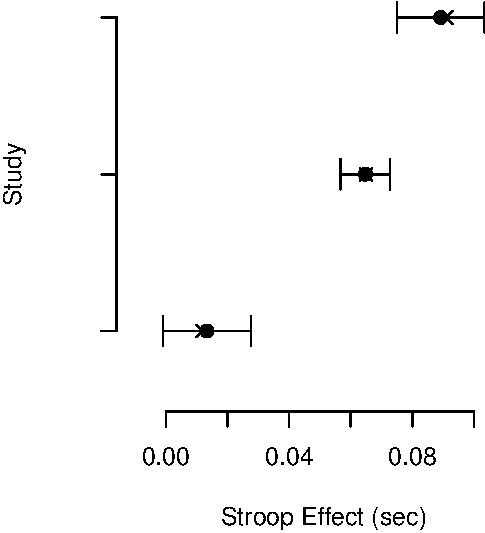
\includegraphics{pBlind_files/figure-latex/hrEst-1.pdf}
\caption{\label{fig:hrEst}Meta-analytic hierarchical-model estimates for
Haaf and Rouder's (2017) collection of Stroop experiments. The effect
varies from study to study, but the sign is consistently positive.}
\end{figure}

Bayes factor analysis reveals that the positive model is most preferred.
It is preferred by a factor of 3.6-to-1 over the unconstrained model, by
a factor of \(10^{11}\)-to-1 over the common-effect model, and by a
factor of \(10^{46}\)-to-1 over the null model.

\section{Corker et al's Stability of the Big Five Personality
Traits}\label{corker-et-als-stability-of-the-big-five-personality-traits}

\begin{figure}[htbp]
\centering
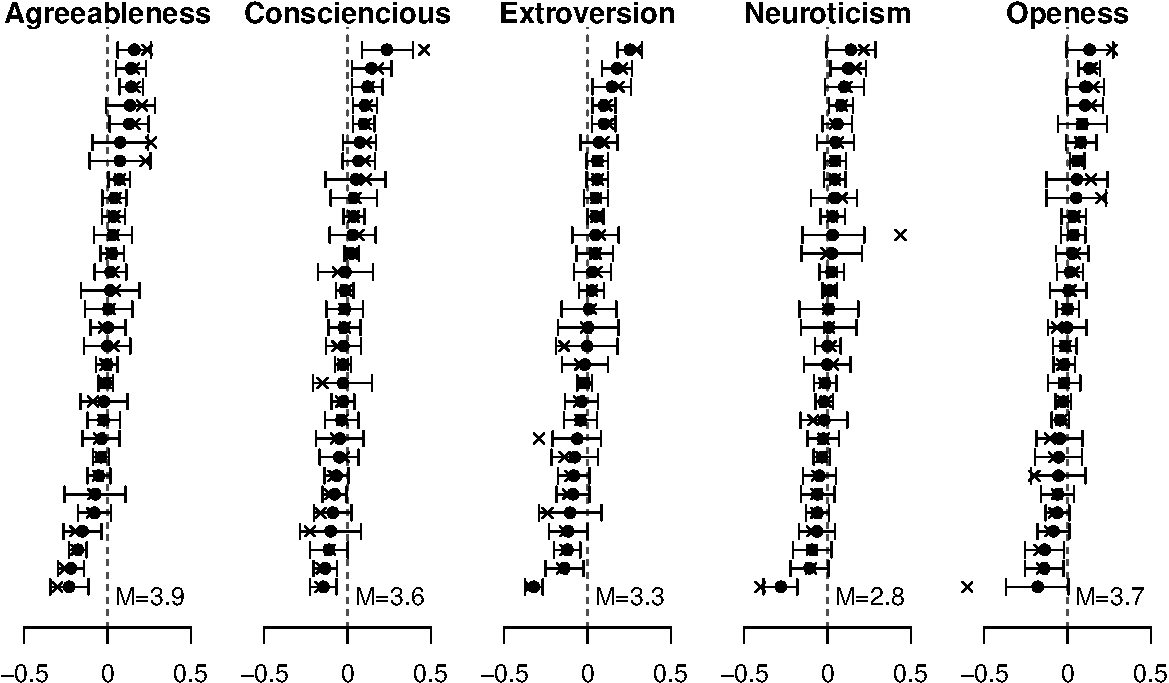
\includegraphics{pBlind_files/figure-latex/corkerEst-1.pdf}
\caption{\label{fig:corkerEst}Meta-analytic hierarchical-model (regularized)
estimates for Big Five personality characteristics across the 30 sites
in Corker et al. (2017). It is apparent that there is substantial
variation across the labs.}
\end{figure}

In the preceding three analyses, the models favored were the null, the
common effect, and the positive effects models. We have yet to find a
meta-analysis where the unconstrained model is preferred to the positive
effects model. We suspect, in fact, that such circumstances are rare in
the literature for well-defined phenomena.

In this section, we reanalyze a recent meta-analysis from Corker et al.
(2017) who examined the stability of personality data from 30 sites.
Their main question is whether the Big Five traits are stable across
different university populations. Big Five traits are measured as Likert
scale ratings of endorsement of certain statements, and each individual
is given a score that ranges from 1 to 5 for each characteristic.
Stability across sites means that the average across people for a
particular trait does not vary across sites. One might hope \emph{a
priori} that site averages do not truly vary as such variation may
complicate personality research.

One feature of the Corker et al. application is that there is no concept
of a true zero, nor are there positive and negative effects. For this
application we focus on models with and without variability across
sites. Corker et al. use a mixed linear model analysis to assess the
variability across sites and to test whether certain covariates, when
included, account for this variability. Their work is exemplary and they
highlight the two themes promoted here: (i). that estimates should be
regularized by models, and (ii). that model comparison and selection is
the primary approach to formally address questions about constraints in
data. Their approach, frequentist mixed modeling, at least in this
application, is similar in spirit to our Bayesian mixed modeling.
Therefore we refit their data as a demonstration that our approach
yields similar conclusions to standard mixed models in cases where order
constraints are not relevant.

To estimate personality traits among labs, we develop a random slope and
intercept estimation model where there are site-specific intercept
parameters and site-specific slope parameters for each personality
trait. For each lab there is a site-specific intercept denoting on
average how people in that lab score across all five factors. If
participants in one lab tend to endorse higher ratings than in another,
the intercept is higher for the first than for the second. There are
also five site-specific personality-characteristic parameters; these are
denoted \(\theta_{ij}\), where \(i\) indexes the site and \(j\) indexes
the personality characteristic \(j=1,\ldots,5\).

The personality parameters are the target of interest. There are two
theoretical positions: one where the distribution of personality traits
is common across sites and another where the distribution indeed varies
across sites. We take the common-effect position first. We constrain
\(\theta_{ij}=\nu_j\), where \(\nu_j\) is a constant that describes how
much of the \(j\)th characteristic there is in the population. To add
heterogeneity across sites\footnote{A formal statement of the models are
  as follows. Let \(Y_{ijk}\) denote the \(k\)th participants score on
  the \(j\)th characteristic in the \(i\)th site. The model is given by
  \(Y_{ijk} \sim \mbox{Normal}(\alpha_i+\theta_{ij},\sigma^2)\) where
  \(\alpha_i\) are site-specific intercepts and \(\theta_{ij}\) are
  defined above. In the common-effect model, the constraint
  \(\theta_{ij}=\nu_j\) guarantees identifiability. In the unconstrained
  model, the constraint
  \(\theta_{ij} \sim \mbox{Normal}(\nu_j,\delta_j)\) is sufficient to
  guarantee identifiability in this context (Rouder et al., 2012).}, we
simply distribute these parameters:
\(\theta_{ij} \sim \mbox{Normal}(\nu_j,\delta_j)\). Here \(\delta_j\) is
the variability across the \(j\)th trait.

Figure~\ref{fig:corkerEst} shows the estimates of \(\bftheta\) from the
unconstrained model. As can be seen, there is a fair amount of
variability for each of the personality characteristics.

There are several approaches to specifying families of models for
comparison. We highlight what we consider to be an appropriate
minimalist approach based on the comparison among three models. The
simplest of these models has slopes and intercepts do not vary across
labs, the second model has intercepts that vary but slopes do that not,
and the third model has intercepts and all five slope parameters that
vary across labs.

The results are as follows: The common intercept and slope model is
least compatible with the data. It is dominated by the unconstrained
intercept and common slope model (Bayes factor of about
\(10^{39}\)-to-1), which is in turn dominated by the unconstrained
intercept and unconstrained slope model (Bayes factor of about
\(10^{48}\)-to-1). These staggering values remain staggering across
reasonable variation in prior settings.

The alternative approach, perhaps a maximalist approach, is to specify
all possible submodels of the unconstrained intercept and slopes model.
Accordingly, we include models where some traits vary across sites while
others do not. An example of such a model is where \emph{agreeableness}
and \emph{openess} vary across sites, but \emph{conscienciousness},
\emph{extraversion}, and \emph{neuroticism} are constant. We have
avoided such models because we have no theoretical basis for testing why
some but not other traits vary across sites. Hence, to us, assessing all
these models is not a well-motivated inferential question. We prefer to
reserve testing (through Bayes factor model comparison) for cases where
models have immediate theoretical interpretations, as they do for the
above three models.

\begin{figure}[htbp]
\centering
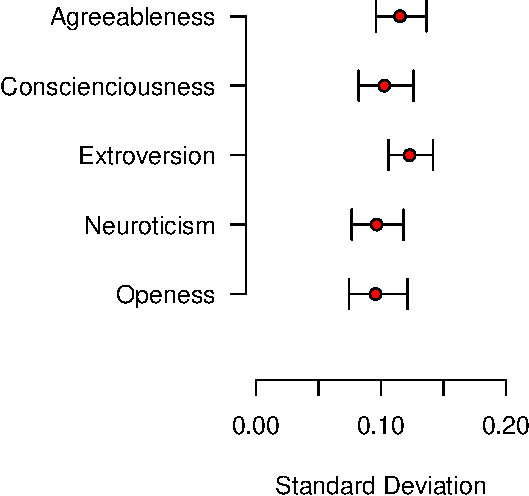
\includegraphics{pBlind_files/figure-latex/corkEst2-1.pdf}
\caption{\label{fig:corkEst2}Estimates of variability of personality
characteristis. Posterior distribution of standard deviations were
computed and plotted are the means and 95\% credible intervals of these
distributions.}
\end{figure}

Even when testing is inappropriate, we may still report estimates of the
variability of the characteristics across the sites.
Figure~\ref{fig:corkEst2} shows the credible intervals on the standard
deviation of personality ratings across sites. As can be seen, the
degree of variability is fairly stable across the characteristics. This
usage of Bayes factor assessment for theoretically important positions
along with estimation for exploration of new phenomena is broadly
useful.

\section{General Discussion}\label{general-discussion}

In this paper, we seek to redefine the fundamental question of
meta-analysis. Traditionally, inferences in meta-analysis are performed
using the mean and CIs. These are properties that help the analyst
understand the distribution of outcomes across a population of
experiments. Yet, we argue this distribution is not well defined, and
properties like mean reflect not only the phenomena under consideration
but how we as a community chose to study it. Moreover, this distribution
is artificial as there is no random sampling process for choosing design
parameters for individual studies.

Here, we suggest focusing on basic ordinal properties that may be shared
in common among all studies in a class. Our null model stipulates that
no study shows an effect. Our common effect model predicts that all
studies have the same common effect. Our positive effects model relaxes
this prediction, stipulating the effect may vary in size, but not in
sign, across studies. We also leave room for the unconstrained case
where some studies show an effect in one direction and others in the
opposite direction. This unconstrained model, if favored, suggests
substantial differences between studies, such that certain methods,
measures, or populations appear to change the sign of the effect. For
laboratory phenomena, success of this unconstrained model should be
cause for careful scrutiny, as even the sign of the effect cannot be
predicted in advance.

\subsection{Advantages and Limitations in Bayesian
Analysis}\label{advantages-and-limitations-in-bayesian-analysis}

The current development is made within the Bayesian framework. There are
a number of reasons we use the Bayesian framework, but perhaps the most
compelling one is that we know of no comparable frequentist development
for the positive-effects model. This model is comprised by placing order
constraints on the true values for each of many studies. Placing a
single order constraint on a linear model is well understood (Robertson,
Wright, \& Dykstra, 1988), but placing tens or hundreds of them (one per
study) simultaneously is not. To our knowledge, although there is a
voluminous frequentist literature on order-constrained inference
(Silvapulle \& Sen, 2011), there are no frequestist tests or model
comparison strategies for the positive effects model vs.~the
unconstrained model. Fortunately, order-constrained inference is
straightforward in the Bayesian framework (Gelfand, Smith, \& Lee, 1992;
Klugkist et al., 2005), and the basic machinery generalizes gracefully
for consideration of many order constraints simultaneously (Haaf \&
Rouder, 2017). Indeed, Bayesian inference has become popular in
statistics because it is tractable in many cases where frequentist
inference is not.

Coarsely speaking, there are two prominent camps or points-of-view in
Bayesian analysis in psychological science. The first camp is the
\emph{estimation camp,} and it is popularized by John Kruschke and
colleagues (Kruschke, 2012; Kruschke \& Liddell, 2017). Here, the goal
is to estimate parameters of interest, and from these estimates, draw
conclusions about the likely relations in the data. The other camp is
the \emph{model comparison} camp, and it is popularized by the Bayes
factor approach (Myung \& Pitt, 1997; Rouder, Speckman, Sun, Morey, \&
Iverson, 2009; Wagenmakers, 2007). Practitioners follow Bayes rule to
derive predictions for models under consideration and compare models by
comparing their predictions. The critical questions here, \enquote{are
all studies null,} or \enquote{are all studies positive,} are best
answered by model comparison. It is unclear what target parameter of
interest one would estimate to assess whether the positive model holds
vs.~its competitors.

One of the key properties we have tried to emphasize in our discourse
are the limitations of testing with Bayes factor model comparison. We
view testing as a powerful tool that must be wielded with expertise,
wisdom, and restraint. Researchers should have well-conceived questions
that are well-instantiated in well-specified models. Not all model
comparisons are helpful and some are even misleading. For example, we
decided to not test variability across each of the Big Five personality
characteristics separately because we were unsure of the theoretical
ramifications of the results.

Another limitation with Bayesian model comparison comes from
considerations in specifying the prior. We expect analysts to differ in
their choices, though these differences should fall in a range of
reasonable values rather than be arbitrarily broad. Restraint is
practiced when we respect this range. In our case, for example, we were
unable to assess whether or not there was variation in prejudice toward
women across sites in Ebersole et al's data set. The conclusion depended
too heavily on how much variation one expected, and different reasonable
values resulted in qualitatively different conclusions. The most prudent
course was to note that the question could not be answered with the data
in hand.

\subsection{Future Directions}\label{future-directions}

We view the development here as only a first step in implementing this
ordinal approach where we ask what is common among a population of
studies. There are many possible extensions that would increase the
usefulness of this approach. One extension is to account for the role of
moderators and other covariates in assessment. We may still assess
whether all studies are positive or null or varied even when
demographics and other covariates are accounted for. Another extension
is to expand the models of incoherent phenomena. Incoherent phenomena
are those where some studies yield truly negative effects while other
studies yield truly positive effects. For these cases, we can stipulate
three classes of studies: those that are negative, null, and positive,
and we can model the distribution of these studies as a three-component
mixture. Each study then has a probability of being in each class.
Moreover, we can assess whether this more flexible model better accounts
for the data than the four presented. Haaf \& Rouder (submitted) have
started making progress on these incoherent mixture models. A third
extension is to model publication bias. Guan \& Vandekerckhove (2016)
provide a new model-based approach, and their treatment of publication
bias may conceivably be incorporated into our meta-analytic models.

We hope this new approach to meta-analysis proves timely and topical.

\newpage

\section*{References}\label{references}
\addcontentsline{toc}{section}{References}

\hypertarget{refs}{}
\hypertarget{ref-Aitkin:1991}{}
Aitkin, M. (1991). Posterior Bayes factors. \emph{Journal of the Royal
Statistical Society. Series B (Methodological)}, \emph{53}(1), 111--142.
Retrieved from \url{http://www.jstor.org/stable/2345730}

\hypertarget{ref-Anderson:etal:2010}{}
Anderson, C. A., Shibuya, A., Ihori, N., Swing, E. L., Bushman, B. J.,
Sakamoto, A., \ldots{} Saleem, M. (2010). Violent video game effects on
aggression, empathy, and prosocial behavior in eastern and western
countries: A meta-analytic review. \emph{Psychological Bulletin},
\emph{136}(2), 151--173. Retrieved from
\url{http://psycnet.apa.org/doi/10.1037/a0018251}

\hypertarget{ref-vanAssen:etal:2015}{}
Assen, M. A. L. M. van, Aert, R. C. M. van, \& Wicherts, J. M. (2015).
Meta-analysis using effect size distributions of only statistically
significant studies. \emph{Psychological Methods}, \emph{20}, 293--309.
Retrieved from \url{http://psycnet.apa.org/doi/10.1037/met0000025}

\hypertarget{ref-Borenstein:etal:2010}{}
Borenstein, M., Hedges, L. V., Higgins, J., \& Rothstein, H. R. (2010).
A basic introduction to fixed-effect and random-effects models for
meta-analysis. \emph{Research Synthesis Methods}, \emph{1}(2), 97--111.

\hypertarget{ref-Carter:etal:2017}{}
Carter, E. C., Schonbrodt, F. D., Hilgard, J., \& Gervais, W. M. (2017).
\emph{Correcting for bias in psychology: A comparison of meta-analytic
methods.} Retrieved from \url{https://osf.io/preprints/psyarxiv/9h3nu/}

\hypertarget{ref-Corker:etal:2017}{}
Corker, K. S., Donnellan, M. B., Kim, S. Y., Schwartz, S. J., \&
Zamboanga, B. L. (2017). College student samples are not always
equivalent: The magnitude of personality differences across colleges and
universities. \emph{Journal of Personality}, \emph{85}(2), 123--135.

\hypertarget{ref-deFinetti:1974}{}
de Finetti, B. (1974). \emph{Theory of probability} (Vol. 1). New York:
John Wiley; Sons.

\hypertarget{ref-Ebersole:etal:2016}{}
Ebersole, C. R., Atherton, O. E., Belanger, A. L., Skulborstad, H. M.,
Allen, J. M., Banks, J. B., \ldots{} Nosek, B. A. (2016). Many labs 3:
Evaluating participant pool quality across the academic semester via
replication. \emph{Journal of Experimental Social Psychology},
\emph{67}, 68--82. Retrieved from
\url{http://ezid.cdlib.org/id/doi:10.17605/OSF.IO/QGJM5}

\hypertarget{ref-Efron:Morris:1977}{}
Efron, B., \& Morris, C. (1977). Stein's paradox in statistics.
\emph{Scientific American}, \emph{236}, 119--127.

\hypertarget{ref-Gelfand:etal:1992}{}
Gelfand, A. E., Smith, A. F. M., \& Lee, T.-M. (1992). Bayesian analysis
of constrained parameter and truncated data problems using Gibbs
sampling. \emph{Journal of the American Statistical Association},
\emph{87}(418), 523--532. Retrieved from
\url{http://www.jstor.org/stable/2290286}

\hypertarget{ref-Gelman:etal:2004}{}
Gelman, A., Carlin, J. B., Stern, H. S., \& Rubin, D. B. (2004).
\emph{Bayesian data analysis (2nd edition)}. London: Chapman; Hall.

\hypertarget{ref-Guan:Vandekerckhove:2016}{}
Guan, M., \& Vandekerckhove, J. (2016). A Bayesian approach to
mitigation of publication bias. \emph{Psychonomic Bulletin and Review},
\emph{23}(1), 74--86. Retrieved from
\url{http://www.cidlab.com/prints/guan2015bayesian.pdf}

\hypertarget{ref-Haaf:Rouder:2017}{}
Haaf, J. M., \& Rouder, J. N. (2017). Developing constraint in Bayesian
mixed models. \emph{Psychological Methods}.

\hypertarget{ref-Haaf:Rouder:submitted}{}
Haaf, J. M., \& Rouder, J. N. (submitted). \emph{Some do and some don't?
Accounting for possible variation in strategies}.

\hypertarget{ref-Jeffreys:1961}{}
Jeffreys, H. (1961). \emph{Theory of probability (3rd edition)}. New
York: Oxford University Press.

\hypertarget{ref-Kass:Raftery:1995}{}
Kass, R. E., \& Raftery, A. E. (1995). Bayes factors. \emph{Journal of
the American Statistical Association}, \emph{90}, 773--795. Retrieved
from
\url{http://amstat.tandfonline.com/doi/abs/10.1080/01621459.1995.10476572}

\hypertarget{ref-Klugkist:Hoijtink:2007}{}
Klugkist, I., \& Hoijtink, H. (2007). The Bayes factor for inequality
and about equality constrained models. \emph{Computational Statistics \&
Data Analysis}, \emph{51}(12), 6367--6379.

\hypertarget{ref-Klugkist:etal:2005}{}
Klugkist, I., Kato, B., \& Hoijtink, H. (2005). Bayesian model selection
using encompassing priors. \emph{Statistica Neerlandica}, \emph{59},
57--69.

\hypertarget{ref-Kruschke:2012}{}
Kruschke, J. K. (2012). Bayesian estimation supersedes the \(t\) test.
\emph{Journal of Experimental Psychology: General}.

\hypertarget{ref-Kruschke:Liddell:2017}{}
Kruschke, J. K., \& Liddell, T. M. (2017). The Bayesian new statistics:
Hypothesis testing, estimation, meta-analysis, and power analysis from a
Bayesian perspective. \emph{Psychonomic Bulletin \& Review}. Retrieved
from \url{http://link.springer.com/article/10.3758/s13423-016-1221-4}

\hypertarget{ref-Monin:Miller:2001}{}
Monin, B., \& Miller, D. T. (2001). Moral credentials and the expression
of prejudice. \emph{Journal of Personality and Social Psychology},
\emph{81}(1), 33.

\hypertarget{ref-Morey:etal:2016}{}
Morey, R. D., Romeijn, J.-W., \& Rouder, J. N. (2016). The philosophy of
Bayes factors and the quantification of statistical evidence.
\emph{Journal of Mathematical Psychology}, --. Retrieved from
\url{http://www.sciencedirect.com/science/article/pii/S0022249615000723}

\hypertarget{ref-Myung:Pitt:1997}{}
Myung, I.-J., \& Pitt, M. A. (1997). Applying Occam's razor in modeling
cognition: A Bayesian approach. \emph{Psychonomic Bulletin and Review},
\emph{4}, 79--95.

\hypertarget{ref-Robertson:etal:1988}{}
Robertson, T., Wright, F., \& Dykstra, R. (1988). \emph{Order restricted
statistical inference.} Wiley, New York.

\hypertarget{ref-Rouder:etal:2017}{}
Rouder, H., J. N. (2017). \emph{From theories to models to predictions:
A bayesian model comparison approach}.

\hypertarget{ref-Rouder:etal:2016b}{}
Rouder, J. N., Morey, R. D., \& Wagenmakers, E.-J. (2016). The interplay
between subjectivity, statistical practice, and psychological science.
\emph{Collabra}, \emph{2}, 6. Retrieved from
\url{http://doi.org/10.1525/collabra.28}

\hypertarget{ref-Rouder:etal:2012}{}
Rouder, J. N., Morey, R. D., Speckman, P. L., \& Province, J. M. (2012).
Default Bayes factors for ANOVA designs. \emph{Journal of Mathematical
Psychology}, \emph{56}, 356--374. Retrieved from
\url{http://dx.doi.org/10.1016/j.jmp.2012.08.001}

\hypertarget{ref-Rouder:etal:2009a}{}
Rouder, J. N., Speckman, P. L., Sun, D., Morey, R. D., \& Iverson, G.
(2009). Bayesian \(t\)-tests for accepting and rejecting the null
hypothesis. \emph{Psychonomic Bulletin and Review}, \emph{16}, 225--237.
Retrieved from \url{http://dx.doi.org/10.3758/PBR.16.2.225}

\hypertarget{ref-Silvapulle:Senn:2011}{}
Silvapulle, M. J., \& Sen, P. K. (2011). \emph{Constrained statistical
inference: Order, inequality, and shape constraints} (Vol. 912). John
Wiley \& Sons.

\hypertarget{ref-Simonsohn:etal:2014}{}
Simonsohn, U., Nelson, L. D., \& Simmons, J. P. (2014). P-curve: A key
to the file-drawer. \emph{Journal of Experimental Psychology: General},
\emph{143}, 534--547. Retrieved from \url{10.1037/a0033242}

\hypertarget{ref-Spiegelhalter:etal:2002}{}
Spiegelhalter, D. J., Best, N. G., Carlin, B. P., \& Linde, A. van der.
(2002). Bayesian measures of model complexity and fit (with discussion).
\emph{Journal of the Royal Statistical Society, Series B (Statistical
Methodology)}, \emph{64}, 583--639.

\hypertarget{ref-Stanley:Doucouliagos:2014}{}
Stanley, T. D., \& Doucouliagos, H. (2014). Meta-regression
approximations to reduce publication selection bias. \emph{Research
Synthesis Methods}, \emph{5}(1), 60--78. Retrieved from
\href{DOI:\%2010.1002/jrsm.1095}{DOI: 10.1002/jrsm.1095}

\hypertarget{ref-Stein:1956}{}
Stein, C. (1956). Inadmissibility of the usual estimator for the mean of
a multivariate normal distributions. In \emph{Proceedings of the third
berkeley symposium on mathematical statistics and probability} (Vol. 1,
pp. 197--206).

\hypertarget{ref-Strack:etal:1988}{}
Strack, F., Martin, L. L., \& Stepper, S. (1988). Inhibiting and
facilitating conditions of the human smile: A nonobtrusive test of the
facial feedback hypothesis. \emph{Journal of Personality and Social
Psychology}, \emph{54}(5), 768--777.

\hypertarget{ref-Vanpaemel:2010}{}
Vanpaemel, W. (2010). Prior sensitivity in theory testing: An apologia
for the Bayes factor. \emph{Journal of Mathematical Psychology},
\emph{54}, 491--498.

\hypertarget{ref-Vanpaemel:Lee:2012}{}
Vanpaemel, W., \& Lee, M. D. (2012). Using priors to formalize theory:
Optimal attention and the generalized context model. \emph{Psychonomic
Bulletin \& Review}, \emph{19}, 1047--1056.

\hypertarget{ref-Veichtbauer:2010}{}
Veichtbauer, W. (2010). Conducting meta-analyses in R with the metafor
package. \emph{Journal of Statistical Software}, \emph{36}(3). Retrieved
from \url{http://www.jstatsoft.org/v36/i03/}

\hypertarget{ref-Wagenmakers:2007}{}
Wagenmakers, E.-J. (2007). A practical solution to the pervasive problem
of p values. \emph{Psychonomic Bulletin and Review}, \emph{14},
779--804. Retrieved from \url{https://doi.org/10.3758/BF03194105}

\hypertarget{ref-Wagenmakers:etal:2016}{}
Wagenmakers, E.-J., Beek, T., Dijkhoff, L., Gronau, Q. F., Acosta, A.,
Adams Jr, R., \ldots{} others. (2016). Registered replication report:
Strack, Martin, \& Stepper (1988). \emph{Perspectives on Psychological
Science}, \emph{11}(6), 917--928.

\hypertarget{ref-Zellner:Siow:1980}{}
Zellner, A., \& Siow, A. (1980). Posterior odds ratios for selected
regression hypotheses. In J. M. Bernardo, M. H. DeGroot, D. V. Lindley,
\& A. F. M. Smith (Eds.), \emph{Bayesian statistics: Proceedings of the
First International Meeting held in Valencia (Spain)} (pp. 585--603).
University of Valencia.






\end{document}
